\documentclass[tikz, border=5pt]{standalone}
\usepackage{amsmath}
\usetikzlibrary{patterns}

\newcommand{\drawgrid}{
    \draw[step=1cm,gray,very thin] (0,0) grid (4,4);
}

\newcommand{\goalstates}[1]{
    \foreach\i in {#1} {
        \pgfmathsetmacro{\x}{mod (\i, 4)}
        \pgfmathsetmacro{\y}{int (\i / 4)}
        \fill[gray!20] (\x, 3-\y) rectangle (\x+1, 4-\y);
        \fill[pattern=north east lines, pattern color=gray!50] (\x, 3-\y) rectangle (\x+1, 4-\y);
    }
}

\newcommand{\fillgrid}[1]{
    \foreach\i [count={\xi} from 0] in {#1} {
        \pgfmathsetmacro{\x}{mod (\xi,4)}
        \pgfmathsetmacro{\y}{int (\xi/4)}
        \node[] at (\x+0.5, 3-\y+0.5) {\i};
    }
}

\begin{document}
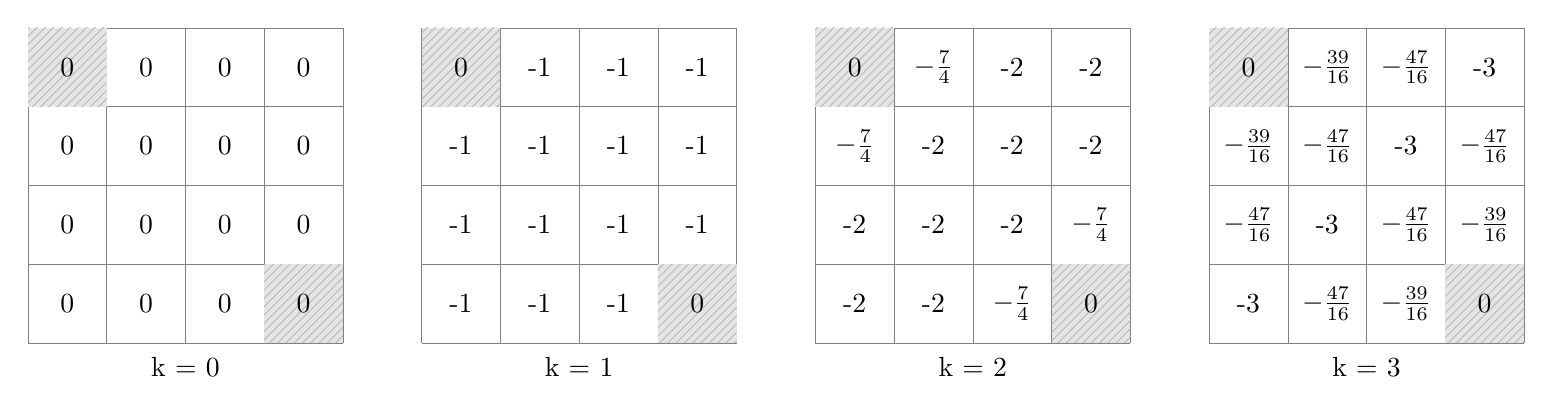
\begin{tikzpicture}

    %% Value iteration
    % k = 0
    \begin{scope}
        \drawgrid
        \goalstates{0, 15}
        \fillgrid{0, 0, 0, 0, 0, 0, 0, 0, 0, 0, 0, 0, 0, 0, 0, 0}
    \end{scope}

    % k = 1
    \begin{scope}[xshift=5cm]
        \drawgrid
        \goalstates{0, 15}
        \fillgrid{0, -1, -1, -1, -1, -1, -1, -1, -1, -1, -1, -1, -1, -1, -1, 0}
    \end{scope}

    % k = 2
    \begin{scope}[xshift=10cm]
        \drawgrid
        \goalstates{0, 15}
        \fillgrid{0, \(-\frac{7}{4}\), -2, -2, \(-\frac{7}{4}\), -2, -2, -2, -2, -2, -2, \(-\frac{7}{4}\), -2, -2, \(-\frac{7}{4}\), 0}
    \end{scope}

    % k = 3
    \begin{scope}[xshift=15cm]
        \drawgrid
        \goalstates{0, 15}
        \fillgrid{0, \(-\frac{39}{16}\), \(-\frac{47}{16}\), -3, \(-\frac{39}{16}\), \(-\frac{47}{16}\), -3, \(-\frac{47}{16}\), \(-\frac{47}{16}\), -3, \(-\frac{47}{16}\), \(-\frac{39}{16}\), -3, \(-\frac{47}{16}\), \(-\frac{39}{16}\), 0}
    \end{scope}

    % Labels
    \node at (2, -0.3) {k = 0};
    \node at (7, -0.3) {k = 1};
    \node at (12, -0.3) {k = 2};
    \node at (17, -0.3) {k = 3};

\end{tikzpicture}
\end{document}
